\chapter{Introduzione}

Questo documento illustra la realizzazione del progetto di \textit{Scalable e Reliable Services}. L'obiettivo è sviluppare un servizio per la previsione degli esiti delle partite di NBA, accessibile tramite un'applicazione web. Inoltre, l'applicazione fornirà informazioni statistiche relative a partite, squadre e giocatori, incluse le quote di scommessa per i mercati head-to-head e spread (head-to-head con handicap).

\section{Architettura}

Di seguito viene descritta l'architettura del sistema, inclusi tutti i componenti e le interazioni tra essi.

\begin{figure}[H]
\centering
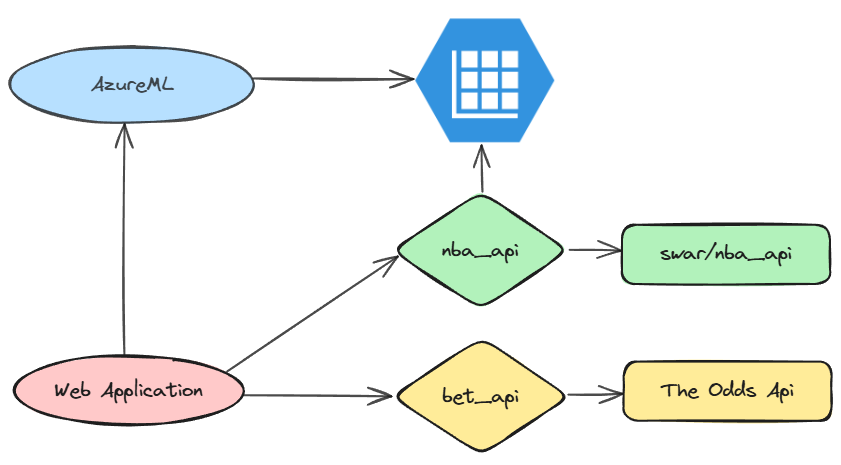
\includegraphics[width=0.9\textwidth]{img/architecture.png}
\caption{Architettura del sistema}
\end{figure}

Ai margini dell'architettura, rappresentati come rettangoli, troviamo due servizi esterni: \texttt{swar/nba\_api}, utilizzato per ottenere informazioni statistiche sulla NBA, e \texttt{The Odds Api}, che fornisce le quote di scommessa aggiornate in tempo reale.

Per facilitare l'uso di questi servizi esterni, sono stati sviluppati due middleware sotto forma di server REST API. Questi middleware offrono endpoint mirati e semplificati per l'interazione con i servizi esterni.

In azzurro, è rappresentato un modello di Machine Learning implementato sulla piattaforma Azure. Questo modello è stato progettato per prevedere l'esito delle partite NBA e viene addestrato utilizzando un database riempito con dati storici delle partite, forniti direttamente dal middleware \texttt{swar/nba\_api}.

Infine, in rosa, troviamo l'applicazione web che interagisce con i due middleware per ottenere le informazioni necessarie da visualizzare e con il modello di Machine Learning per ottenere la predizione dell'esito di una determinata partita.

\vspace{+20px}

Nei capitoli successivi verranno analizzati nel dettaglio tutti i componenti descritti. Inizieremo con i middleware, per poi passare al modello di Machine Learning e infine all'applicazione web.

Nella fase conclusiva, verrà descritto il processo di deployment del servizio in cloud sulla piattaforma Azure, con una spiegazione delle risorse utilizzate e dei costi sostenuti.
